%%
%% This is file `tikzposter-template.tex',
%% generated with the docstrip utility.
%%
%% The original source files were:
%%
%% tikzposter.dtx  (with options: `tikzposter-template.tex')
%% 
%% This is a generated file.
%% 
%% Copyright (C) 2014 by Pascal Richter, Elena Botoeva, Richard Barnard, and Dirk Surmann
%% 
%% This file may be distributed and/or modified under the
%% conditions of the LaTeX Project Public License, either
%% version 2.0 of this license or (at your option) any later
%% version. The latest version of this license is in:
%% 
%% http://www.latex-project.org/lppl.txt
%% 
%% and version 2.0 or later is part of all distributions of
%% LaTeX version 2013/12/01 or later.
%% 


\documentclass{tikzposter} %Options for format can be included here

\usepackage{epsfig}
\usepackage{amsmath}
\usepackage{amssymb}
\usepackage{multicol}

\def\cparam{\mathbf{c}}
\def\R{\mathbb{R}}
\def\N{\mathbb{N}}
\def\Z{\mathbb{Z}}
\def\Q{\mathbb{Q}}
\def\C{\mathbb{C}}
\def\P{\mathbb{P}}
\def\E{\mathbb{E}}
\def\c#1{\mathcal{#1}}
\def\r#1{\text{#1}}
\def\h#1{\widehat{#1}}
\def\b#1{\mathbb{#1}}
\def\t#1{\widetilde{#1}}
\def\on{\mathrm{On}}
\def\1{\mathbbold{1}}
\def\eps{\varepsilon}
\def\diff{\backslash}
\def\d{\mathrm{d}}
\def\pd{\partial}

\def\D{\mathbb{D}}

 % Title, Author, Institute
\title{Connecting two points via random blobs}
\author{Frankie Higgs, fh350@bath.ac.uk}
\institute{Department of Mathematical Sciences, University of Bath}
\titlegraphic{
\includegraphics[scale=2.5]{images/uob-logo-grey-transparent}}

 %Choose Layout
\usetheme{Default}

\begin{document}

 % Title block with title, author, logo, etc.
\maketitle

\block{Abstract}{
Given an open set $A \subseteq \R^d$,
place $n$ iid points distributed according to
a probability distribution $\mu$ on $A$.
At each point, place a ball of radius $r$.
The union of these balls, $Z(n,r)$, is called the \emph{Boolean model},
or the \emph{continuum percolation model}.

When $A$ is bounded, we can ask a whole range of interesting geometric and topological questions: Is a given $B \subseteq A$ completely covered by $Z(n,r)$?
Is $Z(n,r)$ connected? Is it simply connected?
Given two points on the boundary of $A$, is there a path in $Z(n,r)$ connecting them?

We can look at these events as $n \to \infty$
via \emph{event thresholds},
the smallest value of $r$ such that a given event occurs.

Based on work by myself, Mathew Penrose and Xiaochuan Yang.
}
 \begin{columns}

 % FIRST column
\column{0.55}% Width set relative to text width

\block{The Boolean model}{
	Let $A \subseteq \R^d$ be open, and let $\mu$ be a probability measure on $A$.
	Let $\mathcal{X} := (X_1, X_2, \dots)$ be a family of iid points distributed according to $\mu$,
	and for $n \geq 1$ let $\mathcal{X}_n := (X_1, \dots, X_n)$.
	For a given $r > 0$
	let $Z(n,r) := \bigcup_{x \in \mathcal{X}_n} B(x,r)$,
	where $B(x,r) := \{ y \in \R^d : \| x - y \| \leq r \}$.
	We call $Z(n,r)$ the \emph{Boolean model}.
	
	Suppose that $A$ is bounded,
	and take $\mu$ to be normalised Lebesgue measure.
	Without loss of generality also suppose that $A$ has Lebesgue measure 1.
}

\begin{subcolumns}
\subcolumn{0.5}
\block{Coverage events}{
	Let $B \subseteq A$.
	Given $\mathcal{X}_n$,
	the \emph{coverage threshold}
	for $B$ is defined as
	\[
		R_n := \inf\{ r > 0 : B \subseteq Z(n,r) \}.
	\]
	If $\overline{B} \subseteq A$,
	then we can avoid boundary effects.
	The behaviour of the coverage event in this case
	has been understood since the mid 1980s
	\cite{hall85} \cite{janson86}.
	
	In this case, we have the strong law \cite{euclidean-coverage}
	\[
		\frac{n \theta_d R_n^d}{\log n} \to 1
	\]
	almost surely as $n \to \infty$,
	where $\theta_d$ is the volume of a unit ball.
	Note that $n \theta_d R_n^d$ is the total volume of the balls $\{ B(x,R_n) : x \in \mathcal{X}_n \}$.
	% whose union is $Z(n,r)$.
}
\block{}{
\centering
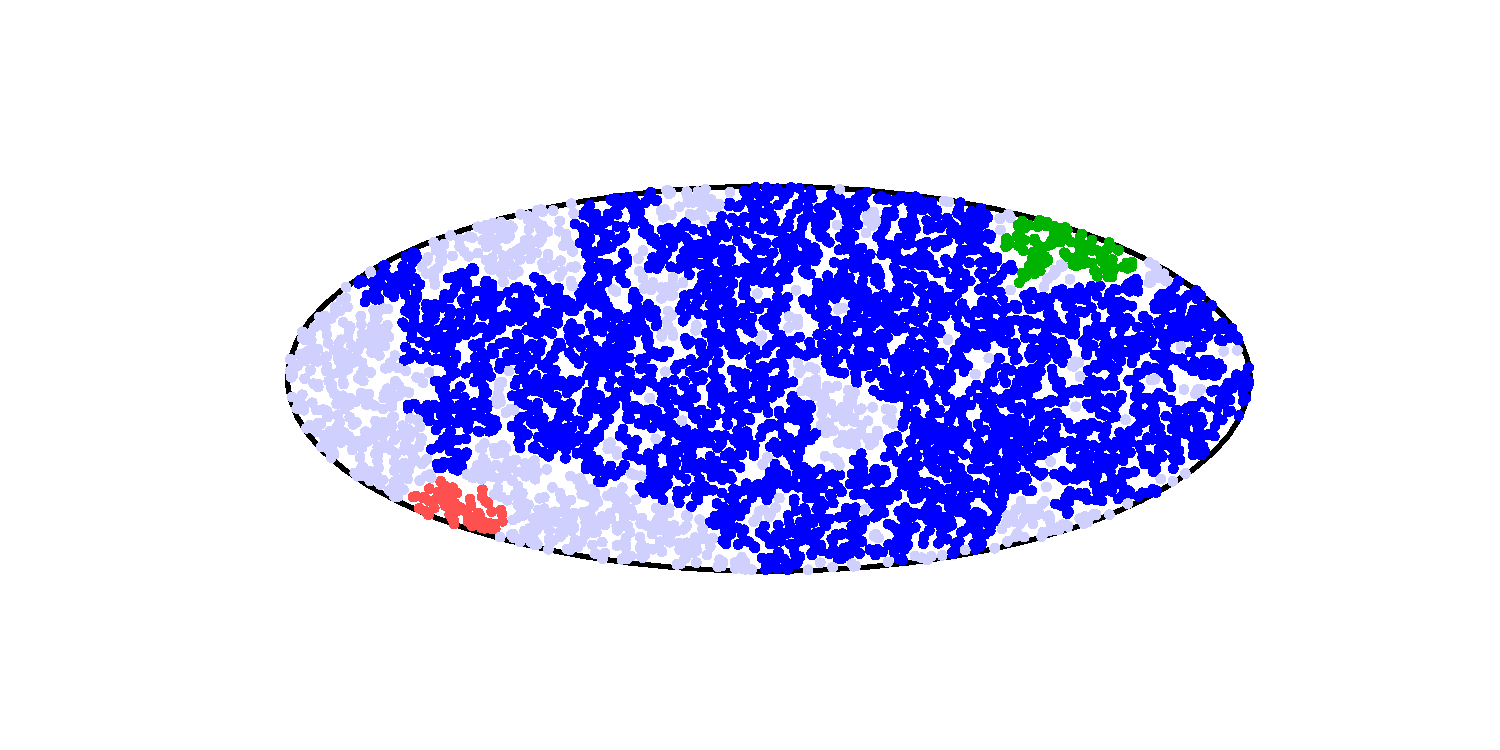
\includegraphics[width=1.0\linewidth, trim=130 80 115 85, clip]{connection-diagram/neither_percolates}
When $\lambda > \lambda_c$,
there will be a giant component.
Above,
neither $x$ nor $y$
is contained in the giant component.
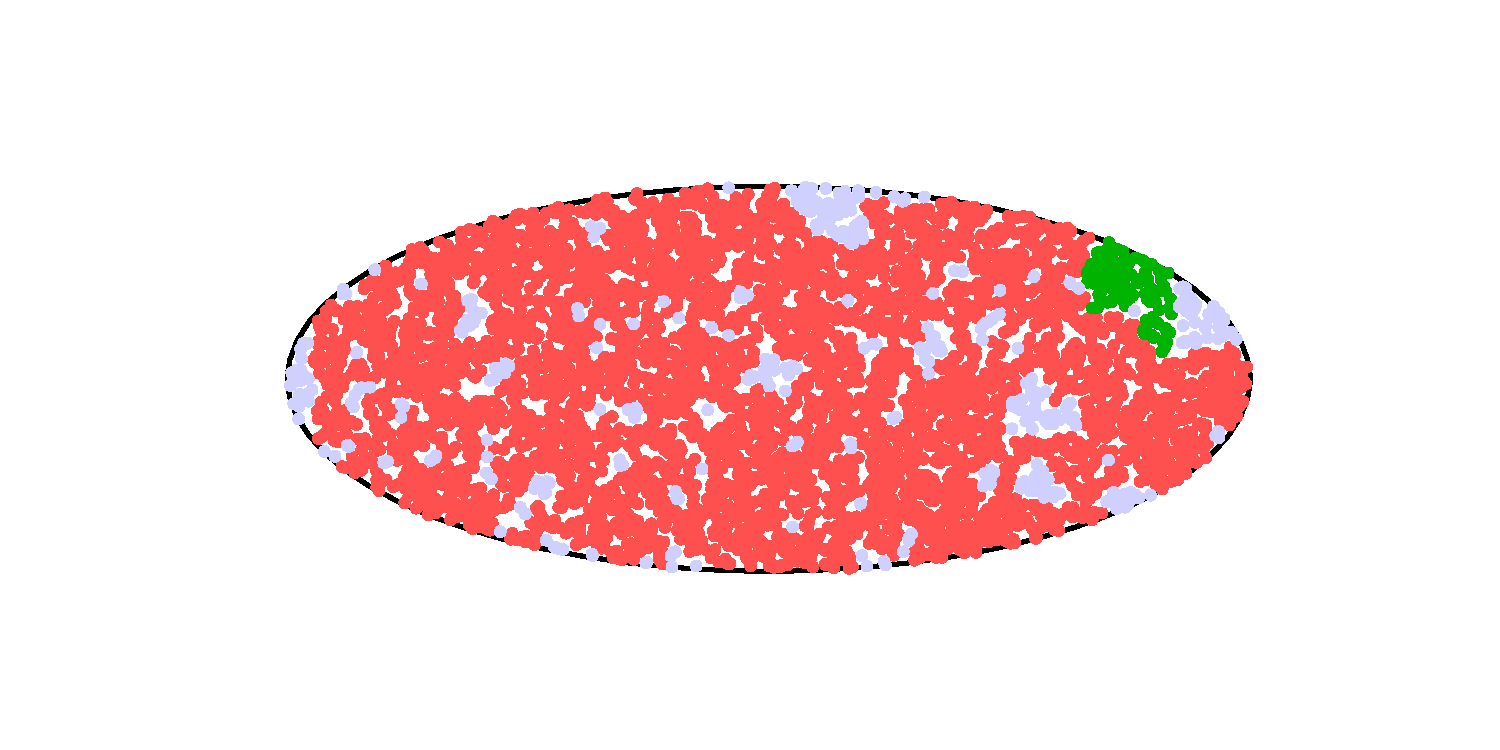
\includegraphics[width=1.0\linewidth, trim=130 80 115 50, clip]{connection-diagram/x_percolates}
$x$ is in the giant component,
but $y$ is not.
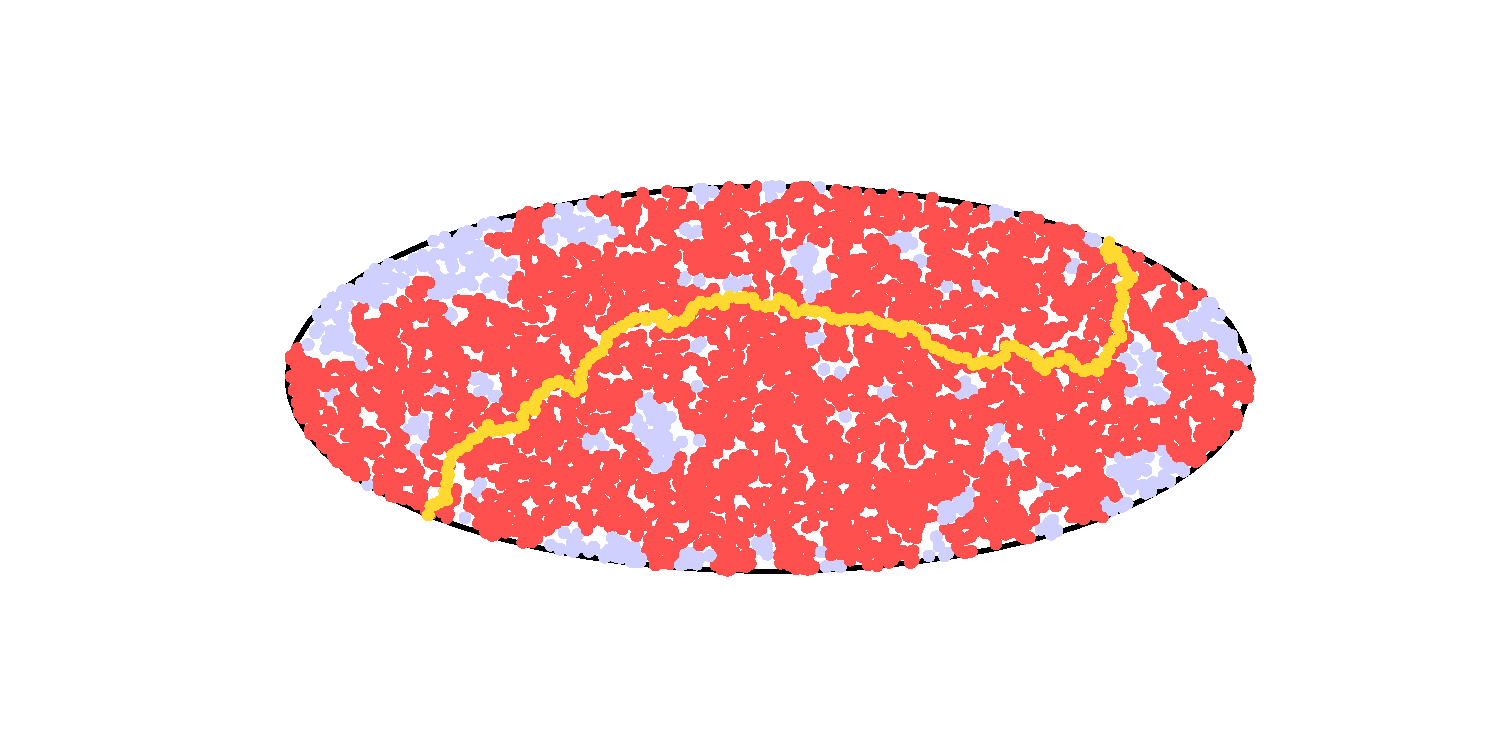
\includegraphics[width=1.0\linewidth, trim=130 80 115 50, clip]{connection-diagram/simple-path}
$x$ and $y$ are connected via the giant component.
}

\subcolumn{0.5}
\block{}{
\centering
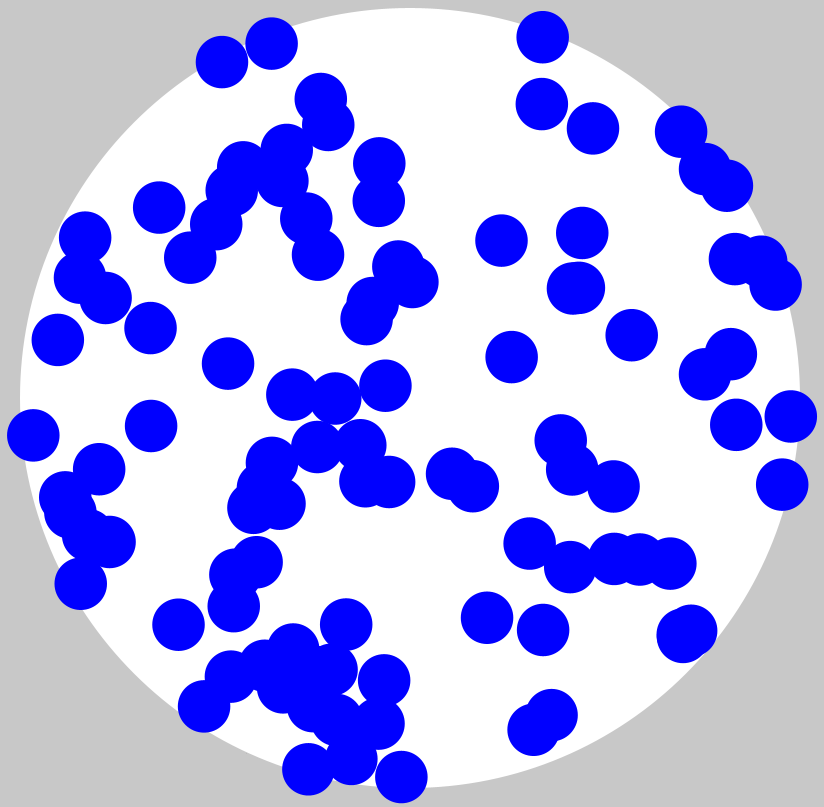
\includegraphics[width=0.23\textwidth]{images/boolean-example}
The Boolean model inside a unit disc
}
\block{Boundary effects}{
	Suppose $B = A$.
	There are two cases:
	(i) $A$ has a smooth boundary, and
	(ii) $A$ is a convex polytope
	with finitely many faces.
	
	In case (i), we have the strong law
	\[
		\frac{n \theta_d R_n^d}{\log n} \to 2 - 2/d
	\]
	almost surely as $n \to \infty$.
	For $d \geq 3$, the limit is greater than 1:
	the furthest point in $\overline{A}$ from $\mathcal{X}_n$
	is close to the boundary $\partial A$.
	
	In case (ii), the strong law \cite{euclidean-coverage}
	 depends on the geometry of $A$.
	We will state the strong law only in the $d = 3$ case:
	if $E$ is the set of edges of the polytope,
	for $e \in E$ let $\alpha_e$ be the angle between the two faces meeting at $e$.
	Let $\alpha_{\mathrm{min}} := \min_{e \in E} \alpha_e$
	be the sharpest angle.
	Then the strong law is
	\[
		\frac{n R_n^3}{\log n} \to \frac{1}{
			\min( \pi, 2 \alpha_{\mathrm{min}} )
		}
	\]
	almost surely as $n \to \infty$.
	
	If $\alpha_{\mathrm{min}} \geq \pi/2$,
	then this is the same limit as in case (i).
	
	There is an interesting phase transition:
	if $\alpha_{\mathrm{min}} > \pi/2$,
	then the furthest point from $\mathcal{X}_n$
	is (asymptotically) uniformly distributed on $\partial A$.
	If $\alpha_{\mathrm{min}} < \pi/2$,
	then the furthest point is (again, in the limit) uniformly distributed
	on all edges $e \in E$ for which $\alpha_e = \alpha_{\mathrm{min}}$.
	
	A similar phase transition exists for all $d \geq 3$.
}
\end{subcolumns}

\block{}{
	Similar results can be proved
	when $A$ is a Riemannian manifold with boundary.
}

 % SECOND column
\column{0.45}

\block{Topological thresholds}
{
	There are other events we can look at,
	such as the topology of $Z(n,r)$.
	Define the \emph{no-holes threshold}
	\[
		V_n := \sup\{ r > 0 : \R^d \setminus Z(n,r) \text{ is not connected} \}.
	\]
	If $A$ is simply connected with a sufficiently smooth boundary,
	or is a convex finite polytope, then $V_n \leq R_n$
	provided $R_n < \eps$ for some constant $\eps > 0$.
	
	In upcoming work we show that the no-holes threshold
	follows the same strong law (with the same limits)
	as the coverage threshold.
}

\block{Percolation-type scaling}{
	The coverage and no-holes events
	only have non-trivial limiting probabilities
	when $n r^d \approx \log n$ as $n \to \infty$.
	But we can consider other scaling regimes.
	
	Let $\lambda > 0$ be a constant,
	and keep $n r^d = \lambda$ constant as $n \to \infty$.
	For a given $x \in A$,
	we can calculate
	\begin{align*}
		\P( x \not\in Z(n,r) )
		&= \P( X_i \not\in B(x,r) \text{ for all } i \leq n )\\
		&= [ 1 - \mathrm{Vol}( B(x,r) \cap A ) ]^n\\
		&\sim \exp\left( -\theta_d \lambda \right)
	\end{align*}
	for large $n$.
	
	In this scaling regime,
	we are interested in properties of $Z(n,r)$
	such as its connectivity,
	the size of the largest cluster,
	and the probability of crossing events.
}

\begin{subcolumns}
\subcolumn{0.36}
\block{}{
\centering
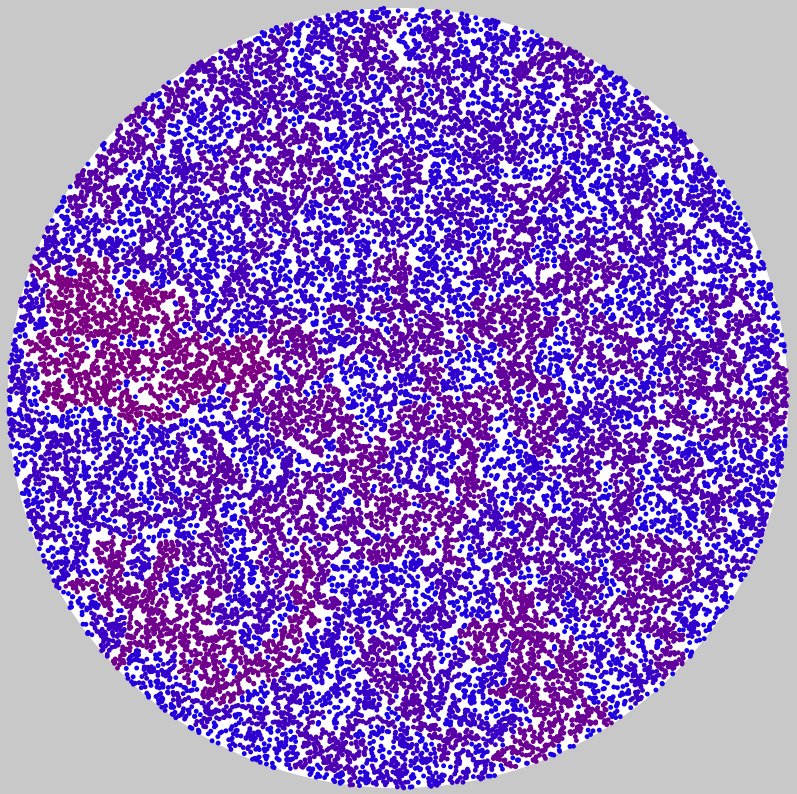
\includegraphics[width=0.12\textwidth]{images/percolation1-0}
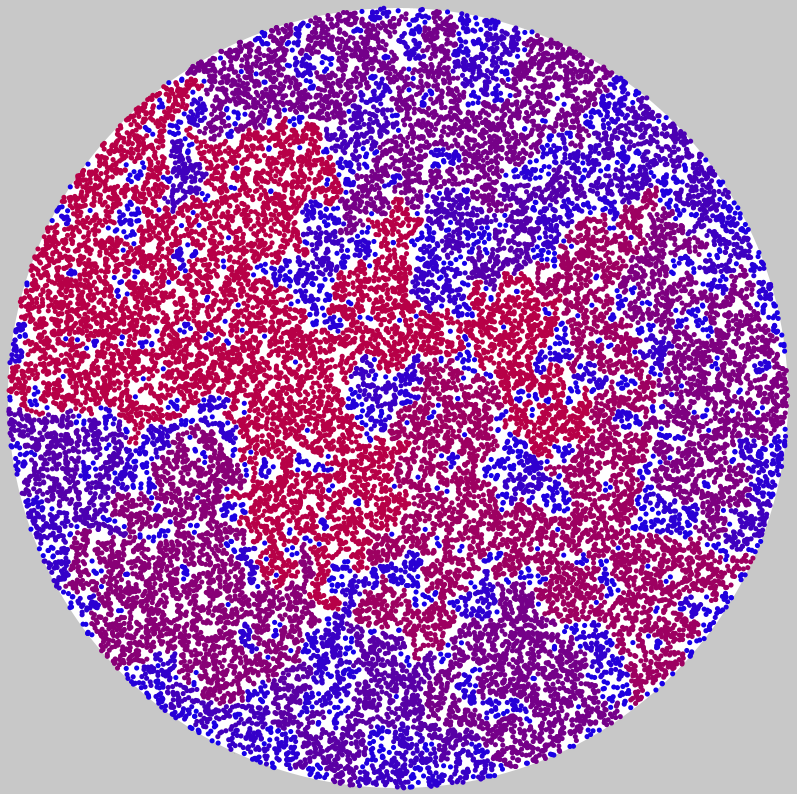
\includegraphics[width=0.12\textwidth]{images/percolation1-1}
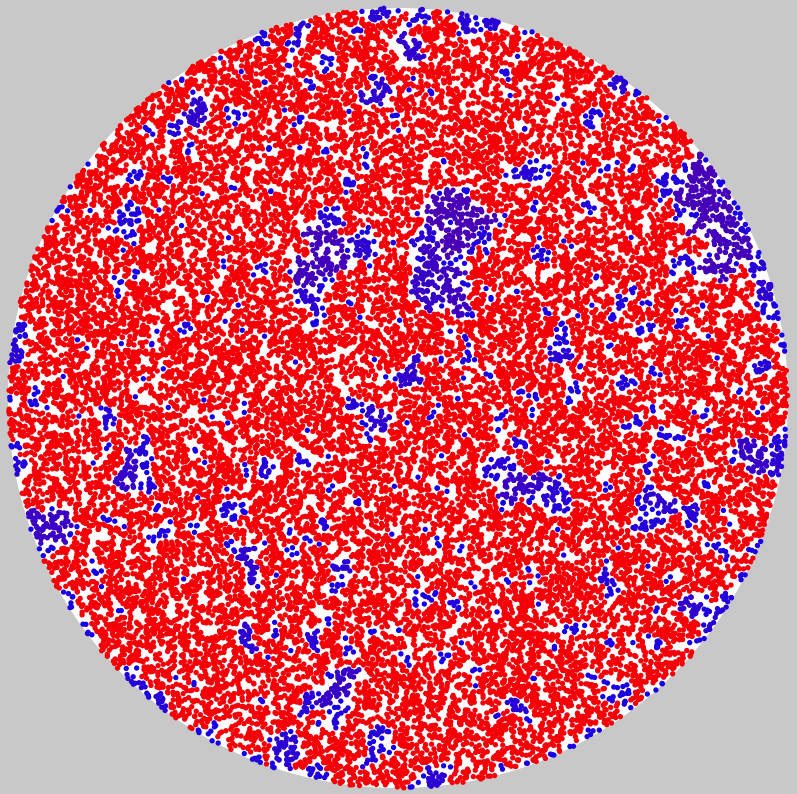
\includegraphics[width=0.12\textwidth]{images/percolation1-2}
}
\subcolumn{0.64}
\block{}{
	Let $x, y \in \partial A$,
	and write $x \leftrightarrow y$
	if there exists a path from $x$ to $y$
	inside $Z(n,r)$.
	
	Let $\theta_{\mathbb{H}}(\lambda)$
	be the percolation probability
	at intensity $\lambda$
	in the half-space $\mathbb{H} := [0,\infty) \times \R^{d-1}$,
	i.e.\ if $\mathcal{P}_\lambda$
	is a homogeneous Poisson point process of intensity $\lambda$ in $\mathbb{H}$,
	and $Z(\lambda) := \bigcup_{x \in \mathcal{P}_\lambda} B(x,1)$,
	then
	$\theta_{\mathbb{H}}(\lambda) := \P[ 0 \leftrightarrow \infty \text{ in } Z(\lambda) ]$.
	
	In upcoming work, we prove that if $\partial A$ is sufficiently smooth,
	then
	$
		\P( x \leftrightarrow y ) \to \theta_{\mathbb{H}}(\lambda)^2
	$
	as $n \to \infty$ with $nr^d = \lambda$.
}

\block{}{
	The above result shows that,
	with high probability,
	long-range connections
	do not exist if $\lambda \leq \lambda_c$,
	where $\lambda_c$ is the critical intensity for half-space percolation,
	and do exist if $\lambda > \lambda_c$.
	
	We expect other percolation-type results
	to also hold for the Boolean model in this scaling regime,
	such as the proportion of the boundary connected to the largest component
	converging to $\theta_{\mathbb{H}}(\lambda)$.
	
	Left:
	this regime
	using the same sample of $\mathcal{X}_n$
	with $\lambda = 1.0$, $1.1$ and $1.2$
	from top to bottom.
	Clusters are coloured according to their size.
}
\end{subcolumns}

\block{}{
\vspace{-40pt}
\bibliographystyle{plain}
\begin{thebibliography}{1}

\bibitem{hall85}
Peter Hall.
\newblock Distribution of size, structure and number of vacant regions in a high-intensity mosaic.
\newblock \textit{Z. Wahrscheinlichkeitstheorie verw Gebiete}, 1985, volume 70, pages 237--261

\bibitem{janson86}
Svante Janson.
\newblock Random coverings in several dimensions.
\newblock \textit{Acta Mathematica}, 1986, volume 156, pages 83--118

\bibitem{euclidean-coverage}
Mathew D. Penrose.
\newblock Random Euclidean coverage from within.
\newblock \textit{Probability Theory and Related Fields}, 2023, volume 185, pages 747--814

\end{thebibliography}
}

\end{columns}



\end{document}

\endinput
%%
%% End of file `tikzposter-template.tex'.
